% Updat
\subsubsection*{Analysis}
\begin{tabular}{@{}l l}
\textbf{Scope}:&
The AuctionHouse\textsuperscript{TM} automated administration system\\
\textbf{Level}:&
User goal\\
\textbf{Primary Actor}:&
Secretary.\\
\textbf{Stakeholders and Interests}:&
\begin{tabular}[t]{@{}l}
Secretary: need it to be quick and easy to update search requests.\\
Buyer: rely on it being correct to find the items they want.
\end{tabular}\\
\textbf{Preconditions}:&
The User has been authenticated.\\
\textbf{Postconditions}:&
\begin{tabular}[t]{@{}l}
The search request has been updated or a failure was returned.\\
\end{tabular}\\
\textbf{Special requirements}:&
The list of search requests on the system.\\
\textbf{Frequency of occurence}:&
Dependant on how often buyers wish to change their search requests.\\
\end{tabular}\\\\
\textsl{Main Success Scenario}
\begin{enumerate}[noitemsep]
	\item The user begins the update search request transaction. % the user requests a search request request request.
	\item The system provides the user with the list of search requests. % the system requests a search request request.
	\item The user provides the system with the Search ID of the request they wish to update. % the user requests a search request
	\item The system provides the user with the updateable parameters of the requested search request.
	\item The user provides the system with all the updated parameters. The parameters that may be updated are:
		\begin{enumerate}[noitemsep]
			\item The item catalogue. 
			\item The maximum price.
		\end{enumerate}
	\item The system updates the search request with the given parameters.
	\item The system returns if it was successful or not.
	 
\end{enumerate}
\textsl{Extensions}
\begin{itemize}[noitemsep]
	\item if unsuccessful the system remains unchanged; no search requests have been added or removed.
\end{itemize}
\textsl{System Sequence Diagram}
\begin{figure}[H]
	\centering
	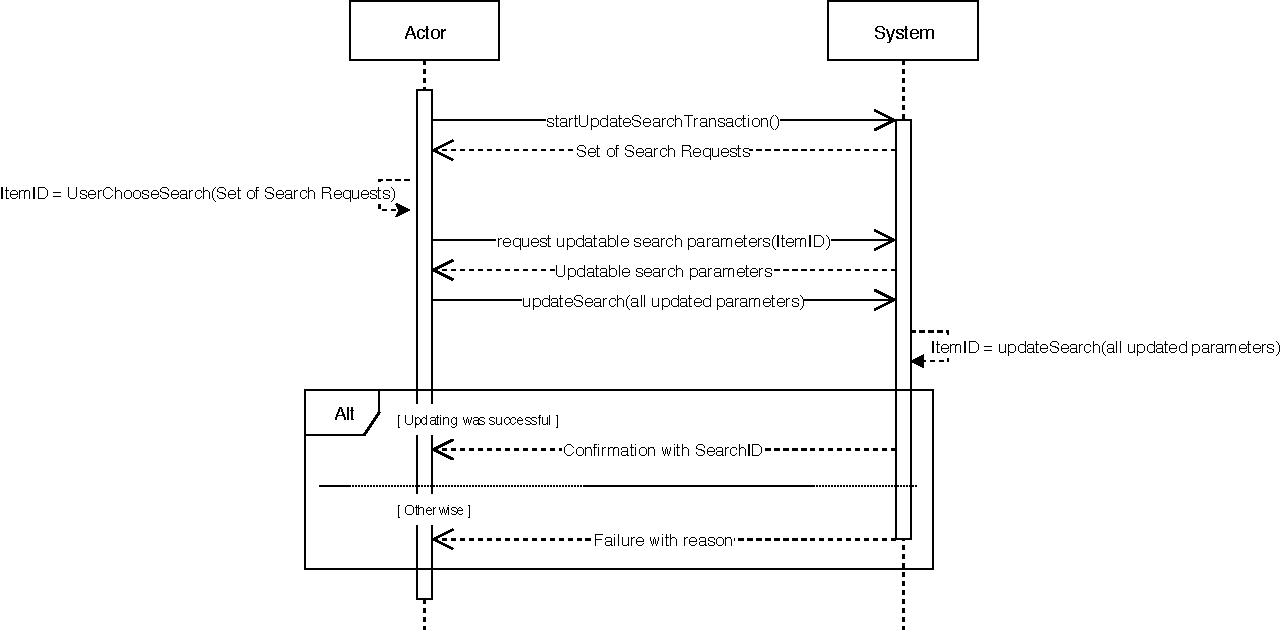
\includegraphics[scale=1]{uml/SD-bb-update-search.pdf}
	\caption*{Interactions displayed in a System Sequence Diagram in blackbox format}
\end{figure}